\documentclass[aspectratio=169]{beamer}

\usetheme{Madrid}
\usecolortheme{default}
\usepackage[utf8]{inputenc}
\usepackage[T1]{fontenc}
\usepackage{graphicx}
\usepackage{booktabs}
\usepackage{amsmath, amssymb}
\usepackage{hyperref}

\title{Wildfire Effects on AQI: What We Learned and How to Use It}
\author{Group 3}
\date{2026-03-09}

\begin{document}

\frame{\titlepage}


\begin{frame}{Business Motivation and Stakeholders}
\textbf{Client}: Air Quality Intelligence Platform \\
\textbf{Stakeholder}: Ontario municipal environmental offices, the Ontario
Ministry of the Environment\\
\textbf{Motivation}: \\
    \begin{itemize}
    \item Explaining extreme AQI events: Tests whether wildfire activity explains AQI spikes missed by baseline models.
    \item Improving forecast reliability: Evaluates whether wildfire features improve next-day AQI predictions, especially on extreme days.
    \item Operational risk signal: Develops a wildfire-aware indicator to support early warnings and air-quality advisories.
    \end{itemize}
\end{frame}


\begin{frame}{Case Study 1 Recap}
\begin{itemize}
    \item Case 1 models performed well on average in predicting next-day AQI using traffic, meteorological, and temporal features. Linear models delivered the best overall performance, but all models struggled to capture episodic spikes in extreme AQI.
    \item The days when our baselines fail are the exact days our users rely on us most for health advisories.
    \item These aligned error spikes are driven by unobserved exogenous factors---specifically, wildfire smoke transport---rather than a lack of model complexity.
\end{itemize}
\end{frame}

\begin{frame}{Business Question}
The key business question is: How can we make next-day AQI forecasts more reliable during high-risk pollution events, particularly during wildfire smoke episodes?

\vspace{0.5em}
More specifically:
\begin{itemize}
    \item Can wildfire activity explain extreme AQI spikes that current models fail to capture?
    \item Can wildfire signals be integrated into the forecasting pipeline to improve advisory reliability?
\end{itemize}
\end{frame}

\begin{frame}{Data Processing Pipeline}
Base Dataset:
\begin{itemize}
\item Case Study 1 station-day AQI dataset
\item CWFIS Fire M3 Daily Hotspots archive (2022--2024)
\end{itemize}

Data Alignment: 
\begin{itemize}
    \item Match weather stations with nearby air quality stations (10 km radius)
    \item Convert hotspots to station-local days; Generate exposure lags (0–3 days)
    \item Merge wildfire features with AQI data; 
    \item Handle missing data by dropping rows with missing targets and using forward fill or station-level median, producing model-ready observations.
    \item Fit the Imputer only on the training data and then transform both training and testing data to avoid data leakage

\end{itemize}
\end{frame}


\begin{frame}{Wildfire Exposure Signal}
\textbf{Wildfire Smoke Exposure Index}

\[
WSEI_{s,t} =
\sum_{f \in F_{t-k}}
\log(1 + I_f)\cdot K(d_{s,f})\cdot W(\Delta \theta_{s,f}, v_s)
\]

\textbf{where}
\begin{itemize}
\item $I_f$: Wildfire intensity (HFI / FRP / TFC)
\item $K(d_{s,f})$: Distance-decay kernel
\item $W(\Delta \theta_{s,f}, v_s)$: Weight hotspots by wind alignment and scale by wind speed
\item $k = 0,1,2,3$ day lags
\end{itemize}
\end{frame}


\begin{frame}{Research Question 1}
After controlling for meteorology, seasonality, and station effects, how strongly is wildfire activity associated with next-day AQI, and over what short lags (0–3 days)?
\end{frame}


\begin{frame}{Modeling Approach}
\begin{itemize}
\item Predict next-day AQI while isolating wildfire effects
\item Incorporate lagged wildfire exposure (0--3 days) to capture smoke transport
\item Control for meteorology, traffic, and calendar structure
\item Hierarchical structure models station-specific baseline AQI levels
\item Bayesian estimation provides uncertainty for wildfire impact
\end{itemize}
\end{frame}

\begin{frame}{Bayesian Estimation}
\textbf{Fitting}
\begin{itemize}
    \item Posterior inference via MCMC (NUTS sampler)
    \item 4 chains $\times$ 2{,}000 iterations (per chain)
\end{itemize}

\textbf{Posterior evidence}
\begin{itemize}
    \item The posterior probability that the cumulative 0--3 day wildfire effect is positive is $> 99.9\%$
\end{itemize}

\textbf{MCMC diagnostics}
\begin{itemize}
    \item R-hat $\approx 1.00$ across parameters (good mixing / convergence)
    \item High effective sample sizes (ESS), suggesting estimates are stable and not driven by sampling noise
\end{itemize}
\end{frame}

\begin{frame}{Wildfire Lag Effect}
\begin{columns}[T]
\column{0.40\textwidth}
 \textbf{Lag-specific Wildfire Effect}: 
 
 Wildfire exposure is associated with higher next-day AQI, with effects concentrated in short lags (0--3 days).

\vspace{2\baselineskip}
\textbf{Cumulative Wildfire Effect}:
    \begin{itemize}
        \item Mean $\approx 4.95$ AQI increase
        \item 95\% credible interval $\approx [4.63, 5.27]$
        \item Probability positive $\approx 1$
    \end{itemize}
\column{0.60\textwidth}
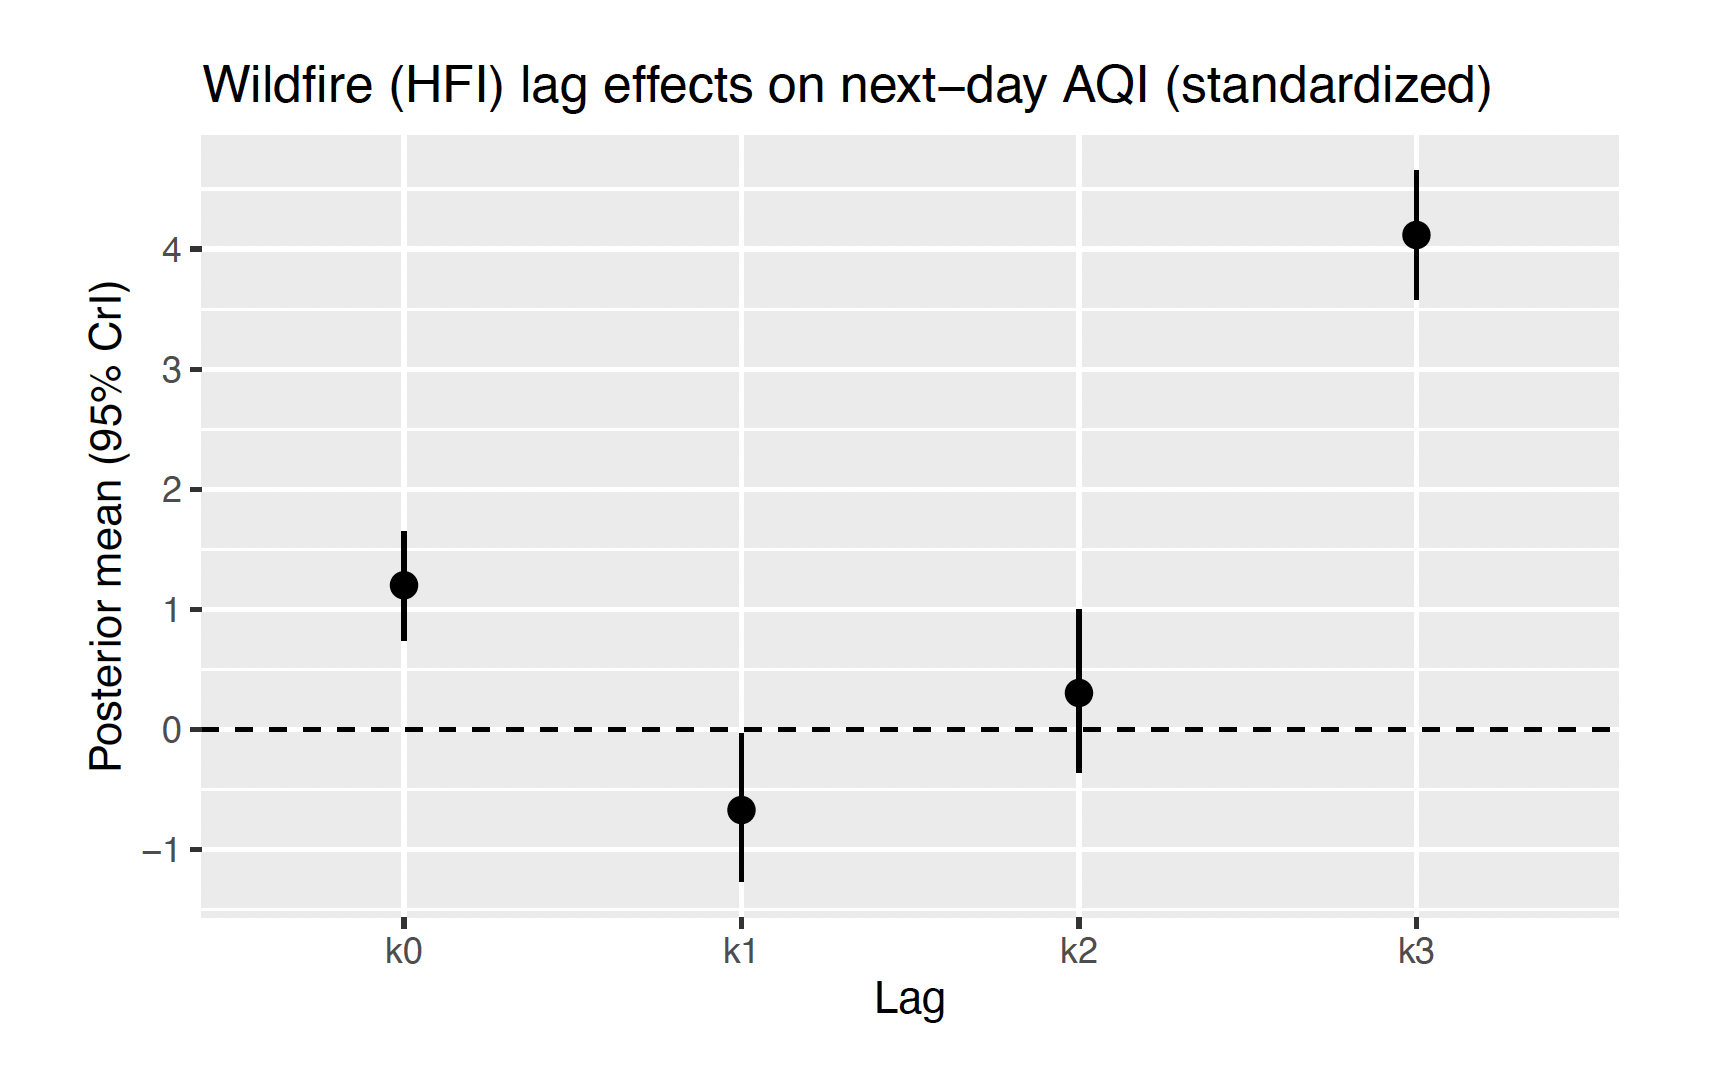
\includegraphics[width=\textwidth]{PresentationImage/LagCoeff.png}
\end{columns}
\end{frame}


\begin{frame}{Posterior Predictive Check}
\begin{columns}[T]
\column{0.5\textwidth}
\begin{itemize}
    \item Model reproduces the main AQI distribution.
    \item Some mismatch in extreme right tail.
    \item Indicates difficulty modeling extreme events.
\end{itemize}

\column{0.5\textwidth}
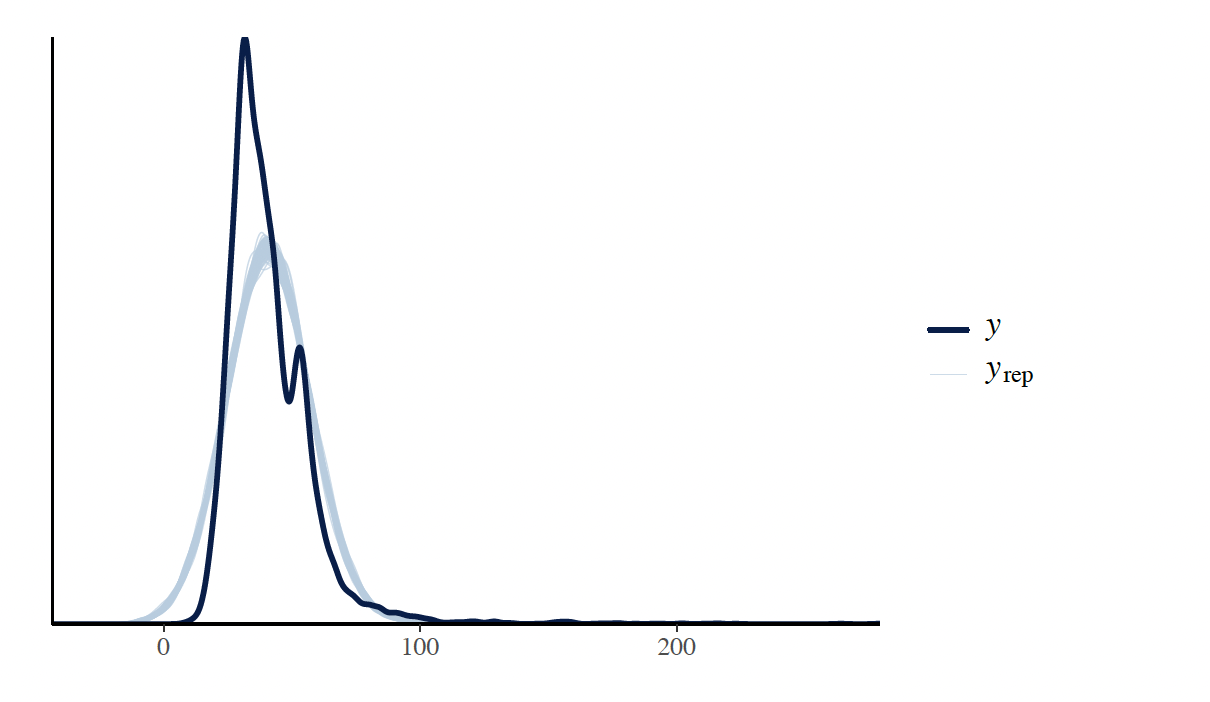
\includegraphics[width=\textwidth]{PresentationImage/PosteriorPred.png}
\end{columns}
\end{frame}

\begin{frame}{Residual Diagnostics}
\begin{columns}[T]
\column{0.40\textwidth}
\begin{itemize}
    \item Residual variance increases at higher AQI levels.
    \item Suggests heteroskedasticity during severe pollution days.
\end{itemize}

\column{0.60\textwidth}
\includegraphics[width=\textwidth]{PresentationImage/residual.png}
\end{columns}
\end{frame}

\begin{frame}{Heavy-Tail Modeling}
\begin{columns}[T]
\column{0.40\textwidth}
\begin{itemize}
    \item Student-$t$ likelihood used to capture extreme pollution spikes.
    \item Estimated degrees of freedom $\approx 3.9$, indicating heavy-tailed AQI distribution.
\end{itemize}

\vspace{0.5em}
\textbf{Key takeaway:}
\begin{itemize}
    \item Strongest wildfire association appears at lag 3, with a clearly positive 95\% credible interval. This likely reflects delayed smoke transport and accumulation in downwind regions before impacting the local AQI.
\end{itemize}

\column{0.60\textwidth}
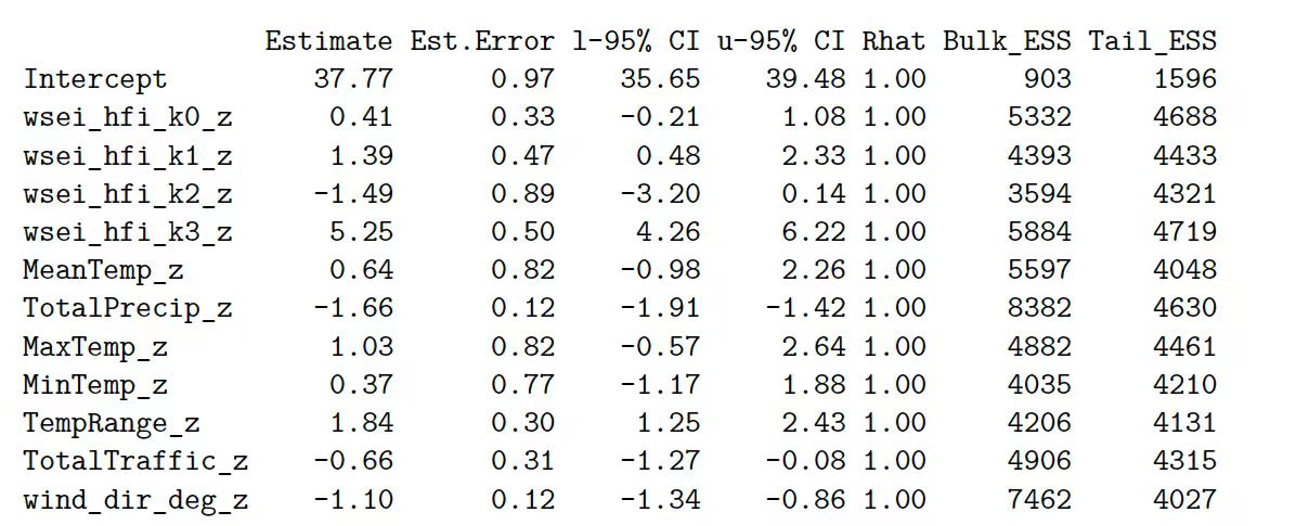
\includegraphics[width=\textwidth]{PresentationImage/TdistCoef.png}
\end{columns}
\end{frame}

\begin{frame}{Gaussian vs Student-$t$}
\begin{itemize}
    \item Gaussian: thin tails $\rightarrow$ extremes inflate $\sigma$ and can distort uncertainty.
    \item Student-$t$: heavy tails (small $\nu$) $\rightarrow$ handles spikes without over-inflating $\sigma$.
    \item Robustness: wildfire lag effects (especially lag 3) stay positive in both models; Student-$t$ is often cleaner/stronger because outliers have less leverage.
\end{itemize}
\end{frame}

\begin{frame}{Remaining Limitations}
\begin{itemize}
    \item Wildfire hotspots are only proxies for smoke transport.
    \item Wind direction treated linearly.
    \item Lag coefficients may trade off due to correlation.
    \item Extreme AQI days remain hard to predict.
\end{itemize}
\end{frame}

\begin{frame}{Research Question 2}
Does adding wildfire exposure features improve next-day AQI point-forecast accuracy, with emphasis on extreme days (e.g., top decile AQI) where Case 1 failed?
\end{frame}

\begin{frame}{Model Comparison Framework}
We compare Baseline vs +Wildfire across three model families:
    \begin{itemize}
        \item OLS
        \item Neural Network (MLP)
        \item LSTM
    \end{itemize}
\end{frame}


\begin{frame}{Model Comparison Results}

\footnotesize

\textbf{Overall performance comparison}

\vspace{0.1cm}
\begin{center}
    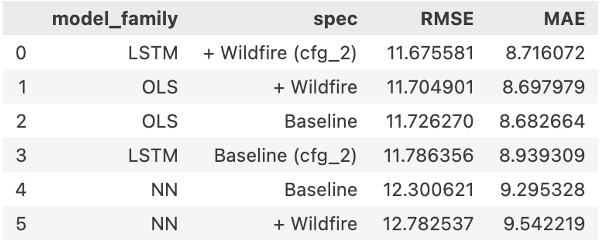
\includegraphics[width=0.5\textwidth]{PresentationImage/RQ2OverallComp.png}
\end{center}

\vspace{0.1cm}

\textbf{Extreme-day performance comparison}

\vspace{0.1cm}
\begin{center}
    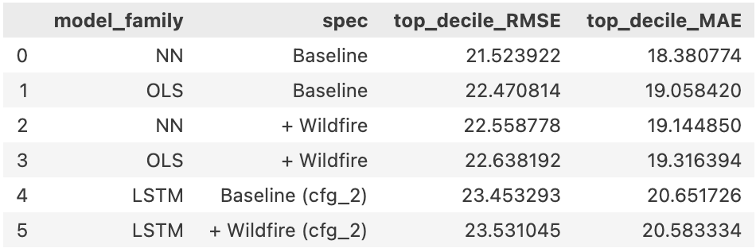
\includegraphics[width=0.5\textwidth]{PresentationImage/RQ2ExtremeComp.png}
\end{center}
\end{frame}

\begin{frame}{Interpretation}
\begin{itemize}
    \item Overall: OLS $\approx$ LSTM; NN worse.
    \item Extreme days: NN baseline best; +Wildfire slightly worse (all models).
    \item Business: no strong smoke-day lift; avoid over-claim.
    \item Action: deploy OLS baseline; wildfire for monitoring/explanation.
    \item Next: transport-aware features; extreme-focused training.
\end{itemize}
\end{frame}

\begin{frame}{Research Question 3}
Can we produce a stable, interpretable wildfire-risk signal (feature + diagnostics) that supports stakeholder-facing explanations and monitoring?
\end{frame}

\begin{frame}{Define the Operational Signal}
\begin{itemize}
    \item Operational target: ``High AQI tomorrow'' event.
    \item Definition: next-day AQI in the top 10\% (binary outcome).
    \item Why this helps stakeholders: a single number for alerts + dashboards.
\end{itemize}
\end{frame}

\begin{frame}{Procedures}
\begin{columns}[T]
\column{0.40\textwidth}
\textbf{Step 1: Define the Monitored Outcome}

Create a binary ``high-AQI tomorrow'' event (top 10\% of next-day AQI).

\vspace{0.5em}
\textbf{Step 2: Fit an Interpretable Risk Model}

Train a Bayesian hierarchical logistic regression.

The model's wildfire exposure features, especially the 3-day lag, meaningfully increase the probability of a high-AQI day tomorrow.

\column{0.60\textwidth}
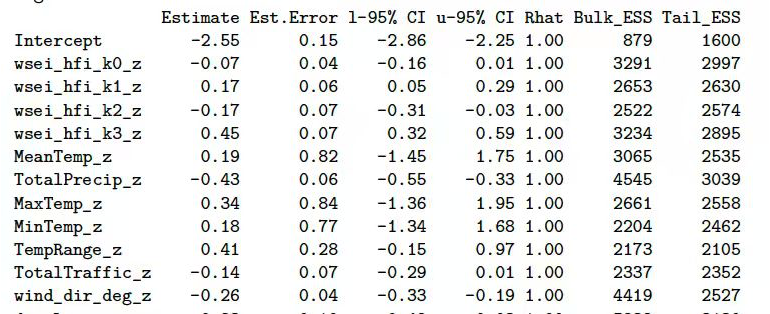
\includegraphics[width=\textwidth]{PresentationImage/RQ3Coeff.png}
\end{columns}
\end{frame}

\begin{frame}{Result: Wildfire Increases High-AQI Risk}
\begin{itemize}
    \item Focus on the most actionable term: lag-3 wildfire exposure ($k_3$).
    \item Coefficient (log-odds): $\approx 0.45$.
    \item Odds ratio: $\exp(0.45) \approx 1.57$.
    \item $\rightarrow \sim 57\%$ higher odds of a high-AQI day per $+1$ SD wildfire exposure.
    \item Interpretation: strongest risk signal appears with $\sim 3$-day delay.
\end{itemize}
\end{frame}

\begin{frame}{Diagnostic A: Calibration of the Risk Score}

\begin{columns}[T]
\column{0.40\textwidth}
\begin{itemize}
    \item Bin predictions into deciles of probability of high AQI next day.
    \item Near-diagonal points $\rightarrow$ probabilities are reasonably calibrated.
\end{itemize}
\column{0.60\textwidth}
\includegraphics[width=\textwidth]{PresentationImage/Calibration.png}
\end{columns}

\end{frame}

\begin{frame}{Diagnostic B: Wildfire-driven Risk Uplift}
\[
\Delta = P(\text{High AQI} \mid \text{WSEI}) - P(\text{High AQI} \mid \text{WSEI} = 0)
\]

\begin{columns}[T]
\column{0.40\textwidth}
\begin{itemize}
        \item mass near 0 $\rightarrow$ wildfire has little effect on most days (good: fewer false alarms)
        \item positive tail $\rightarrow$ wildfire meaningfully increases risk on smoke-impacted days
\end{itemize}

\column{0.60\textwidth}
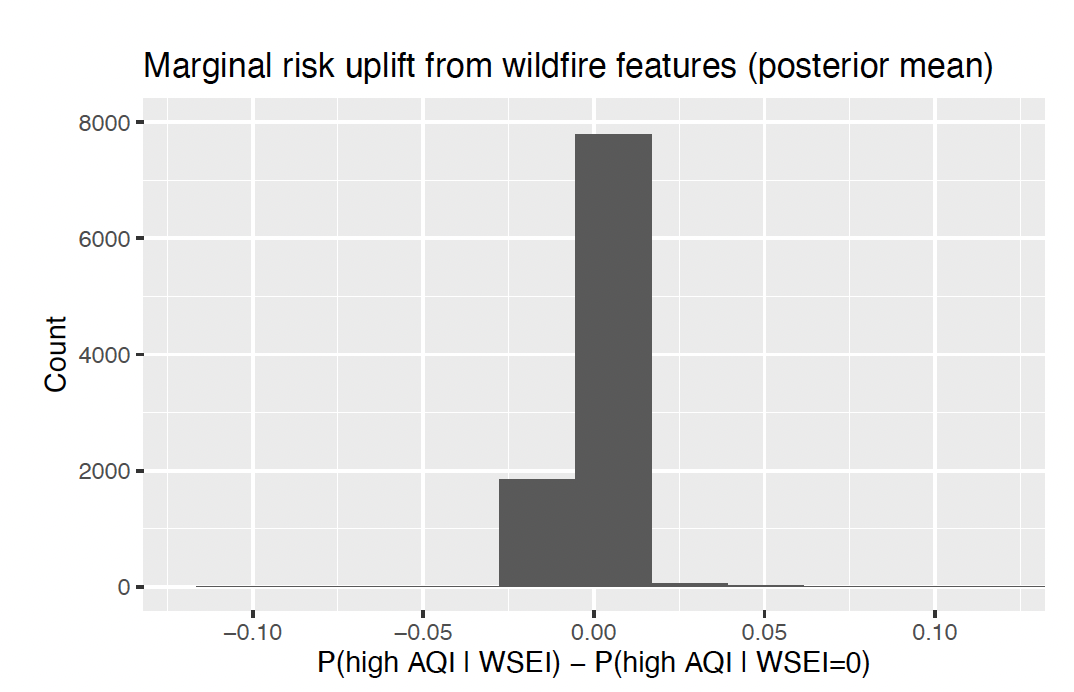
\includegraphics[width=\textwidth]{PresentationImage/RiskUplift.png}
\end{columns}
\end{frame}

\begin{frame}{Conclusion}
\begin{itemize}
    \item Wildfire exposure is positively associated with next-day AQI, with the strongest effect at about a 3-day lag; results are robust under both Gaussian and Student-$t$ errors.
    \item Adding WSEI improves performance during high-AQI periods by explaining spike days that baseline models tend to miss.
    \item The Bayesian risk model provides an interpretable probability score for top-decile AQI events; wildfire features, especially lag-3, raise predicted risk mainly on a limited subset of days.
\end{itemize}

\vspace{0.5em}
\textbf{Value to decision-making}
\begin{itemize}
    \item We can deploy a wildfire-aware early-warning indicator for Ontario: a daily risk probability + a clear explanation of why risk is elevated.
\end{itemize}
\end{frame}

\end{document}
